\documentclass[extendedabs]{recpad2k}
\usepackage{float}

\title{Authority\\ Secure Serverless P2P Chat}

% Enter the paper's authors in order
% \addauthor{Name}{email/homepage}{INSTITUTION_CODE}
\addauthor{João Marques, 2192637}{https://github.com/Yvtq8K3n/Authority}{1}
\addauthor{João Jorge, 2190373}{https://github.com/cloropower}{1}

% Enter the institutions
% \addinstitution{Name\\Address}
\addinstitution{
 Instituto Politécnico de Leiria\\
 Leiria, Portugal
}

\runninghead{Student, Prof, Collaborator}{RECPAD Author Guidelines}

% Any macro definitions you would like to include
% These are not defined in the style file, because they don't begin
% with \bmva, so they might conflict with the user's own macros.
% The \bmvaOneDot macro adds a full stop unless there is one in the
% text already.
\def\eg{\emph{e.g}\bmvaOneDot}
\def\Eg{\emph{E.g}\bmvaOneDot}
\def\etal{\emph{et al}\bmvaOneDot}

%------------------------------------------------------------------------- 
% Document starts here
\begin{document}

\maketitle

\begin{abstract}

Communication is gaining importance and influencing people all around the world, it's important to assure its safety.

There are currently a wide variety of applications that support a secure communication, however most require a third party participation.

Our solution focused on only using the elements necessary for a secure communication.
\end{abstract}

\section{Introduction } 
\label{sec:intro}

Nowadays communication has gained a fundamental weight in the various sociocultural, economic and political areas. The high criticality of communication impulsionated the appearance of various solutions mainly based on a client-server architecture that requires the participation of third parties. This participation, in addition to having additional costs, puts at risk the security of the information. There are also some peer-to-peer solutions such as Skype, pTox that allow communication without third parties, but do not guarantee anonymity. Our solutions wants to solve both problems. It's based on a Peer-to-Peer (P2P) architecture and is intended to remove third party participation, in a way that reduces costs, increases speed and mitigate some of the potential information security risks. Communication is carried out only at the network level, in order to mitigate the anonymity problem.

\section{Fundamental Concepts}
\label{sec:Fundamental Concepts}
In this section Fundamental Concepts it explore all the concepts needed to understand the options adopted in developing the solution.

\subsection{Architecture}
Architecture is one of the fundamental aspects in the development of any software.
In distributed systems the architecture is based in the premise of roles and well defined responsibilities, as follows:


\subsubsection{\em Client-Server}

In the Client Server, roles and responsibilities are well defined, illustrated in {\bf Figure 1}.

\begin{figure}[hp]
\centering
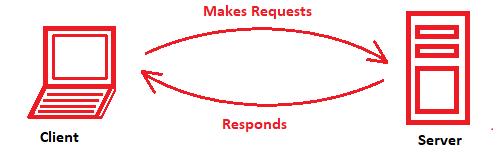
\includegraphics[scale=.50]{images/client-server.png}
\caption{Architecture {\em Client-Server}}
\end{figure}

In this architecture, the client corresponds to the sender of the message and the server is responsible for delivering to the appropriate recipient(s),

\subsubsection{\em Peer-to-Peer}

The {\em Peer-to-Peer} architecture is based on the premise that all the members of the nertwork, denominated by nodes, are the same[2], illustrated in {\bf Figure 2}.

\begin{figure}[H]
\centering
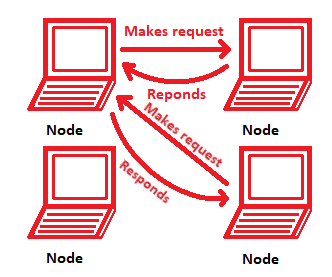
\includegraphics[scale=.50]{images/peer-to-peer.png}
\caption{Peer-to-Peer Architecture}
\end{figure}

There are currently a large set of variations of {\em Peer-to-Peer}, namely:
\begin{itemize}
  \item {\em Structured P2P}, nodes find each other through an hashing table.
  \item {\em Hybrid P2P}, some nodes have more responsibilities than others.
  \item {\em Pure P2P}, all nodes have the same level of responsibility.
  \item {\em Centralized P2P}, a central entity is required in order to management the nodes on the network;
\end{itemize}

Between all the options we chose Pure P2P due to its simplicity and the great advantages it provides. In Pure P2P the communication is made directing from the sending node to the destiny node.

\subsection{\em Network}
The purpose of {\em network} is to enable the communication of information in distributed systems.
A network can be established regardless of the transmission medium (cable, fiber), infrastructure (routers, switch) or associated software. \cite{Tanenbaum}
{\em networks} can be characterized according to is dimension, as follows:
\begin{itemize}
  \item {\em Personal area networks (PANs)}
  \item {\em Local area networks (LANs)}
  \item {\em Wide area networks (WANs)}
  \item {\em Metropolitan area networks (MANs)}
\end{itemize}

Our solution is based on a {\em LAN} which has the advantage of making direct connections between the elements of the same network segment, thus preventing message routing or redirecting through the Internet.

\subsection{Routing}
Routing is the process of selecting a network path for traffic redirection in which can employ the following delivery methods:

\begin{figure}[H]
\minipage{0.16\textwidth}
  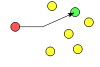
\includegraphics[width=\linewidth]{images/100px-Unicast.png}
  \caption{Unicast}\label{fig:awesome_image1}
\endminipage\hfill
\minipage{0.16\textwidth}
  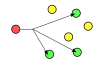
\includegraphics[width=\linewidth]{images/100px-Multicast.png}
  \caption{Multicast}\label{fig:awesome_image2}
\endminipage\hfill
\minipage{0.16\textwidth}%
  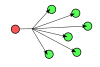
\includegraphics[width=\linewidth]{images/100px-Broadcast.png}
  \caption{Broadcast}\label{fig:awesome_image3}
\endminipage
\end{figure}

In order to process the introduction of a node in the network, it was necessary to develop a protocol that allowed the identification of existing nodes in the network. For this, the {\em Broadcast} and  {\em Unicast} delivery methods applied on the {\emData Link Access} layer were used.

\subsection{Cryptography}

{\em Cryptography is the practice and study of techniques for secure communication in the presence of third parties. (Ronald L, 1990). } \cite{Ronald}

\subsubsection{Symmetric Cryptography}

Symmetric Cryptography is based on the use of the same cryptographic key for message encryption and decryption.

\begin{figure}[hp]
\centering
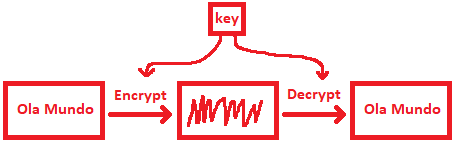
\includegraphics[scale=.50]{images/symetric.png}
\caption{Symmetric Cryptography}
\end{figure}

This type of encryption is computationally light, fast and causes little latency on the network.


\subsubsection{Asymmetric Cryptography}

Asymmetric encryption, also known as public key cryptography, uses a complementary key pair. Both keys allow the processes of encryption and decryption of messages, however only with the other key its possible to reverse the operation performed. Generally the private key is kept secret while the public key is usually distributed.

\begin{figure}[hp]
\centering
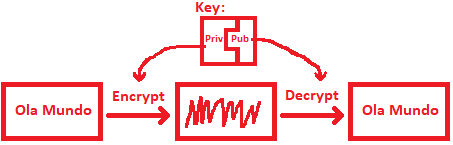
\includegraphics[scale=.50]{images/assymetric.png}
\caption{Asymmetric Cryptography}
\end{figure}

This cryptographic method is extremely computationally heavy and limited, but has the ability to create a secure channel that is difficult to attack.

\section{Proof of Concept}
In this section, all the processes inherent to the idealization and implementation of the developed solution will be explored.

\subsection{Data structure}

In a Peer to Peer network there the needs to exist an identification mechanism of peers. For this, the class {\bf Contact} was developed, which can easily be distributed by the network, being composed of the following properties:

\begin{itemize}
  \item {\em ID}, identification number;
  \item {\em PC-NAME}, name of the computer in the network;
  \item {\em MAC}, network card identification;
  \item {\em IP}, last connected ip address;
  \item {\em Public-key}, public asymmetric key that allows the creation of a secure channel.
\end{itemize}
The information contained in a {\bf Contact} only allows it to be identified it on the network, so a data structure capable of storing all known contacts and ensuring their persistence is required.
For this, based on the ssh protocol the following files were created:

\begin{itemize}
  \item rsa/private,  stores only the private key(s);
  \item rsa/public, stores known contacts, including your own;
 
\end{itemize}

Additionally, given that not all Contacts are available all the time, there is a in memory data structure {\bf Hashmap} that maps the active nodes of the network and list them so the user can create a connection,


\subsection{Introduction on the Network}
One of the major problems with the architecture {\em  Pure Peer to Peer} is the process of introducing a node into the network and the ability of the network to adapt to it. For this, it was necessary to develop a protocol that will be explained below.

\subsubsection{Introduction}
In the introduction process, the new node must demonstrate its intention to join the network, in order to do that, it sends its Contact in {\em Broadcast} via {\em UDP} protocol .

\begin{figure}[hp]
\centering
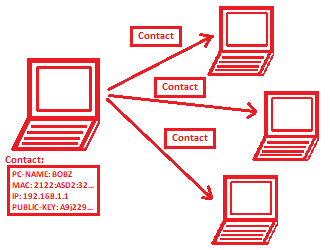
\includegraphics[scale=.50]{images/introducao.png}
\caption{Introduction of Contact}
\end{figure}
    
\subsubsection{Interpretation}
In the interpretation step, each active node in the network processes the new contact, applying the following changes:
\begin{itemize}
  \item rsa/public, add/change corresponding entry;
  \item hashmap, maps new node as active in the network;
\end{itemize}

\begin{figure}[hp]
\centering
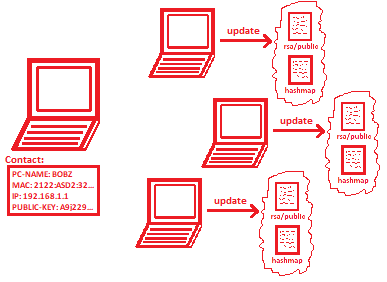
\includegraphics[scale=.50]{images/interpretation.png}
\caption{Processing New Contact}
\end{figure}
 
\subsubsection{Integration}
In the integration process each node after processing the new contact, sends through the {\em TCP} protocol a {\em Unicast} with its own contact, in order to establish a possible future connection.

\begin{figure}[H]
\centering
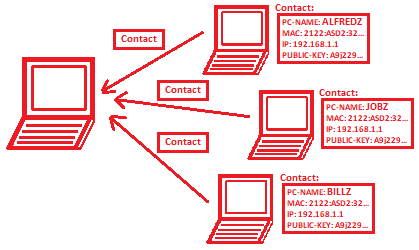
\includegraphics[scale=.50]{images/integration.png}
\caption{Integration of new Contact}
\end{figure}

\subsection{Communication}
After identifying the active nodes in the network, the application allows the creation of communication channels.

\subsubsection{Creation of a Secure Channel}
In order to initialize a communication it is necessary to generate a secure channel. For this, we used the receiver's public key and the emitter's private key, shown in {\bf Figure~\ref{fig:Secure Channel}}.

\begin{figure}[H]
\centering
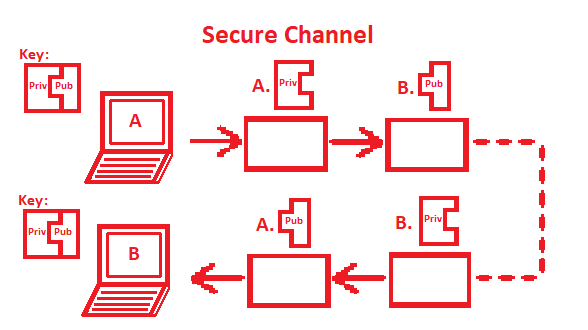
\includegraphics[scale=.50]{images/SecureChannel.png}
\caption{Creation of a Secure Channel}
\label{fig:Secure Channel}
\end{figure}

The receiver in order to obtain the information sent in the secure channel, must reverse the process sender used, that is, use the private key and then the public key of the sender.
This channel is secure, however it is based on asymmetric cryptography which is not ideal.

\subsubsection{Key Exchange}
Using the previously generated secure channel, the emitter node generates a symmetric key and sends it.
This symetric key will be used from now on, until the communication is finished.

\subsection{Tests}
In this chapter some of the tests carried out to ensure the normal functioning of the application will be addressed.

\subsubsection{Node Recognition}
To carry out this test, the computer "Desktop-QUACKMAN" started the application. It applied the Introduction process, but since there was no node on the network, no contacts were added. This process is shown in Figure {\ref{fig:Contactos}}.

\begin{figure}[H]
\centering
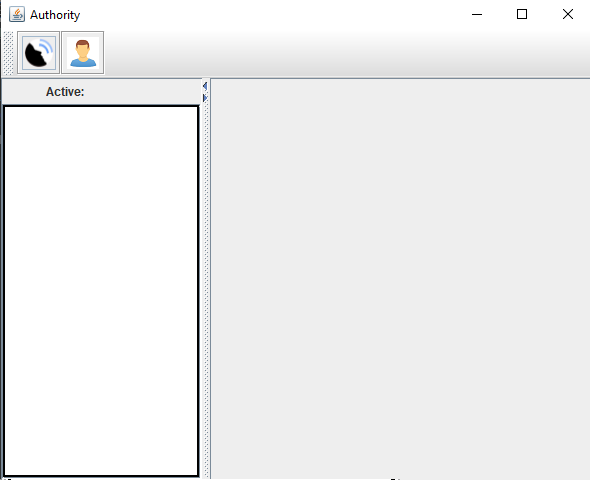
\includegraphics[scale=.30]{images/teste_quackman_contacts.png}
\caption{Contacts of DESKTOP-QUACKMAN}
\label{fig:Contactos}
\end{figure}

Then the computer "Desktop-Marquez" opens the application and both computers update their contacts as expected.

{\bf Note:} During this test, we verified that firewalls can block the process of identifying elements on the network.

\begin{figure}[H]
\centering
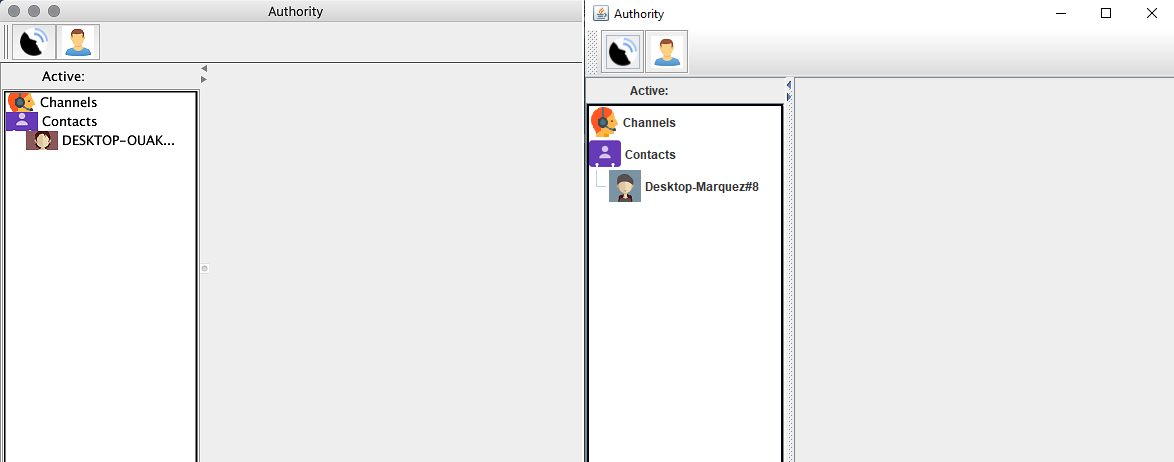
\includegraphics[scale=.30]{images/teste_both_contacts.png}
\caption{Contacts of both computers}
\end{figure}

\subsubsection{Creation of a Communication}
DESKTOP-QUACKMAN selects the contact joaos-mbp.lan. The application creates a corresponding channel in "Channel", shown in {\bf Figure ~\ref{fig:Channel Creation}}.

\begin{figure}[H]
\centering
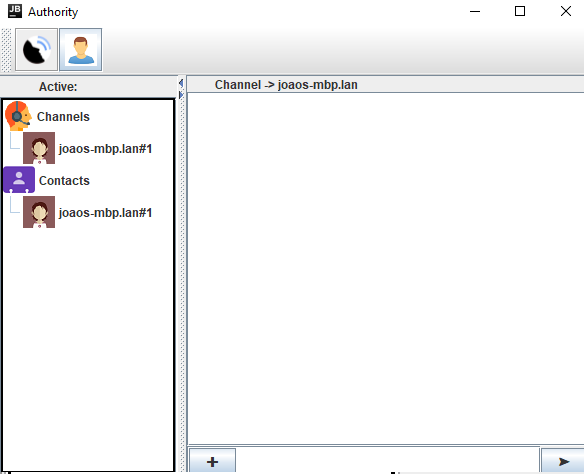
\includegraphics[scale=.30]{images/teste_channels.png}
\caption{Creation of a Channel}
\label{fig:Channel Creation}
\end{figure}

\subsubsection{Chat Conversation}
The user DESKTOP-QUACKMAN, after creating a channel, exchanges messages with the user joaos-mbp.lan.

\begin{figure}[H]
\centering
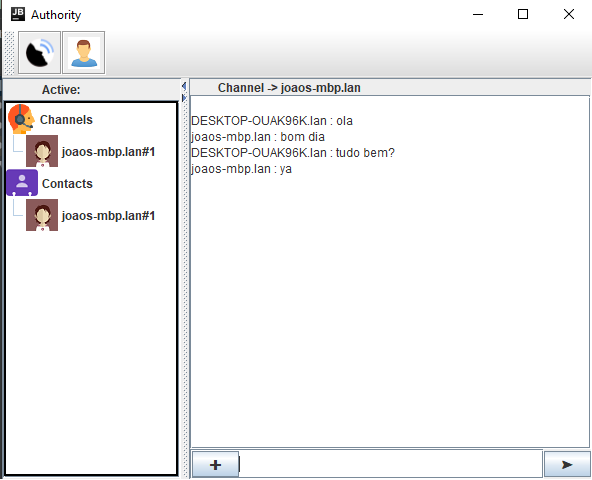
\includegraphics[scale=.30]{images/teste_chat_funcional.png}
\caption{Example of chat usage}
\label{fig:Utilização Chat}
\end{figure}

\subsection{Discussion of Results}
Initially, the use of certificates for identifying nodes on the network was considered. However, due to their creation, sharing and storage, it became an unfeasible option. The non-use of certificates prevented the use of the secure communication protocol TLS/SSH, so it was necessary to create the entire infrastructure that would allow its creation.

To circumvent the problem, Java's Crypto library was used, which allows the creation of various types of symmetric and/or asymmetric keys. Due to the way the RSA algorithm works, it prevented the successive application of the encryption process, thus making it difficult to create the secure channel.

To get around this situation, it was necessary to split the bytes resulting from the first encryption into two parts and apply a second encryption to each.

We had to apply this process because of the way the RSA encryption algorithm itself works, which, being a {\em Block Cipher}, the encryption result always produces a set of bytes with a minimum size.

Unfortunately, it was not possible to complete the file upload and download process via chat.

\subsection{Conclusion}

With the elaboration of this work it was possible to learn about distributed architectures and in detail the variations of Peer to Peer.

Additionally, it was possible to gain experience with the use of cryptographic algorithms, namely RSA and AES.

We suggest continuing this type of work since it allows us to explore in some detail certain technologies and areas taught in the Curricular Unit.

\bibliography{egbib}
\end{document}